\documentclass[12pt,addpoints]{repaso}
\grado{6}
\nivel{Primaria}
\cicloescolar{2024-2025}
\materia{Matemáticas}
\unidad{3}
\title{Practica la Unidad}
\aprendizajes{\scriptsize%
% \item Estudio de los números.
\item Expresa oralmente la sucesión numérica hasta billones, en español y hasta donde sea posible, en su lengua materna, de manera ascendente y descendente a partir de un número natural dado. Ordena, lee y escribe números naturales de más de nueve cifras e interpreta números decimales en diferentes contextos. Identifica semejanzas y diferencias entre el sistema de numeración decimal y otros sistemas como el maya y el romano\\[-1.5em]
	% \item Suma y resta, su relación como operaciones inversas.
	\item A partir de situaciones problemáticas vinculadas a diferentes contextos, suma y resta números decimales y fracciones con diferentes denominadores.\\[-1.5em]
	% \item Multiplicación y división, su relación como operaciones inversas.
	\item Resuelve situaciones problemáticas vinculadas a diferentes contextos que implican dividir números decimales entre naturales. También, dividir números fraccionarios entre números naturales.\\[-1.5em]
	% \item Relaciones de proporcionalidad.
	\item A partir de situaciones problemáticas de proporcionalidad vinculadas a diferentes contextos, determina valores faltantes en las que en ocasiones se conoce el valor unitario y en otras no.\\[-1.5em]
	% \item Ubicación espacial.
	\item Lee, interpreta y elabora planos para comunicar la ubicación de seres vivos y objetos.\\[-1.5em]
	% \item Figuras y cuerpos geométricos y sus características.
	\item Explora y reconoce las características del cilindro y cono; anticipa y comprueba desarrollos planos que permiten construirlos.\\[-1.5em]
	% \item Perímetro, área y noción de volumen.
	\item Resuelve situaciones problemáticas que implican calcular el perímetro y área de figuras compuestas por triángulos y cuadriláteros. Resuelve problemas que implican construir, estimar y comparar el volumen de cuerpos y prismas rectos rectangulares mediante el conteo de cubos, y reconoce que existen diferentes cuerpos con el mismo volumen.\\[-1.5em]
	% \item Organización e interpretación de datos.
	\item Interpreta información cuantitativa y cualitativa contenida en tablas, gráficas de barras y circulares para responder preguntas vinculadas a diferentes contextos; construye gráficas de barras. Genera y organiza datos, determina la moda, la media aritmética y el rango para responder preguntas vinculadas a diferentes contextos.\\[-1.5em]
	% \item Nociones de probabilidad.
	\item Clasifica eventos de diversos contextos utilizando términos como seguro, imposible, probable, muy probable o poco probable que sucedan.
}
\author{Melchor Pinto, JC}
\begin{document}
\INFO\afterpage{\blankpage}%

\begin{multicols}{2}
	\tableofcontents
\end{multicols}

\begin{questions}\large

	\addcontentsline{toc}{section}{Unidad 3}
	\section*{Unidad 3}

	\addcontentsline{toc}{subsection}{Estadística y gráficas}
	\subsection*{Estadística y gráficas}

	\addcontentsline{toc}{subsubsection}{Mediana y moda}
	\subsubsection*{Mediana y moda}
	
	\addcontentsline{toc}{subsubsection}{Promedio}
	\subsubsection*{Promedio}

	\questionboxed[2]{Determina la mediana, la moda y el promedio en los siguientes conjuntos de datos:

		\begin{multicols}{2}
			\begin{parts}
				\part 80, 82, 85, 88, 90, 88, 91, 85, 95, 88, 88, 97, 100. \\[1em]
				El promedio es: \fillin[$89$][0.4in]. \\
				La mediana es: \fillin[$88$][0.4in].\\
				La moda es: \fillin[$88$][0.4in].  \\

				\part Los puntajes obtenidos en un juego son: 54, 55, 59, 61, 77, 58, 55, 71, 59, 55, 60, 53, 56 y 60 puntos. \\[1em]
				El promedio es: \fillin[$59.5$][0.4in]. \\
				La mediana es: \fillin[$58.5$][0.4in].\\
				La moda es: \fillin[$55$][0.4in]. \\
				% La desviación media es: \fillin[$4.5$][0.4in].

				\part 22, 25, 21, 23, 29, 30, 28, 27, 23, 26. \\[1em]
				El promedio es: \fillin[$25.4$][0.4in]. \\
				La mediana es: \fillin[$25.5$][0.4in].\\
				La moda es: \fillin[$23$][0.4in].\\
				% La desviación media es: \fillin[$2.6$][0.4in].

				\part Las estaturas de un grupo de personas son: 170, 168, 169, 171, 168, 172, 168, 171 y 173 cm. \\[1em]
				El promedio es: \fillin[$170$][0.4in]. \\
				La mediana es: \fillin[$170$][0.4in].\\
				La moda es: \fillin[$168$][0.4in]. \\
			\end{parts}
		\end{multicols}
	}

	\addcontentsline{toc}{subsubsection}{Interpretación de gráficas}
	\subsubsection*{Interpretación de gráficas}

	\questionboxed[2]{Los resultados de una encuesta se muestran en la siguiente gráfica de barras:

		\begin{multicols}{2}
			\begin{parts}\normalsize
				\part ¿Cuántas personas participaron en la encuesta? \fillin[95][1.5cm]
				\part  ¿Cuál es la fruta menos preferida por las personas? \fillin[naranja][1.5cm]
				\part  ¿Cuál es la fruta preferida por las personas? \fillin[manzana][1.5cm]
				\part ¿Cuántas personas prefieren a las \textit{manzanas}.\fillin[29][1.5cm]
				\part ¿Cuántas personas prefieren a los \textit{plátanos}.\fillin[21][1.5cm]
				\part ¿Cuántas personas prefieren a las \textit{naranjas}.\fillin[19][1.5cm]

				\columnbreak%

				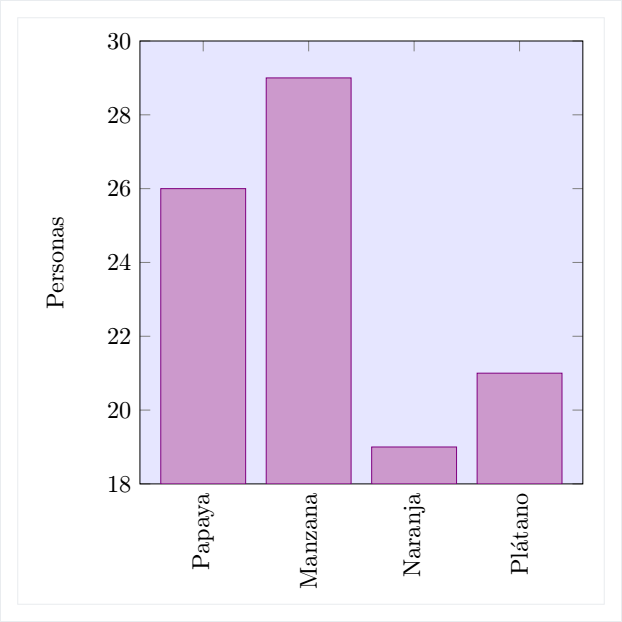
\includegraphics[width=\linewidth]{../images/imagen_barras_frutas01.png}
			\end{parts}
		\end{multicols}

	}

	\questionboxed[2]{Los resultados de una encuesta se muestran en la siguiente gráfica de barras:

		\begin{multicols}{2}
			\begin{parts}\normalsize
				\part ¿Cuántas personas participaron en la encuesta? \fillin[70][1.5cm]
				\part  ¿Cuál es la fruta menos preferida por las personas? \fillin[papaya][1.5cm]
				\part  ¿Cuál es la fruta preferida por las personas? \fillin[plátano][1.5cm]
				\part ¿Cuántas personas prefieren a las \textit{manzanas}.\fillin[16][1.5cm]
				\part ¿Cuántas personas prefieren a los \textit{plátanos}.\fillin[21][1.5cm]
				\part ¿Cuántas personas prefieren a las \textit{naranjas}.\fillin[19][1.5cm]

				\columnbreak%

				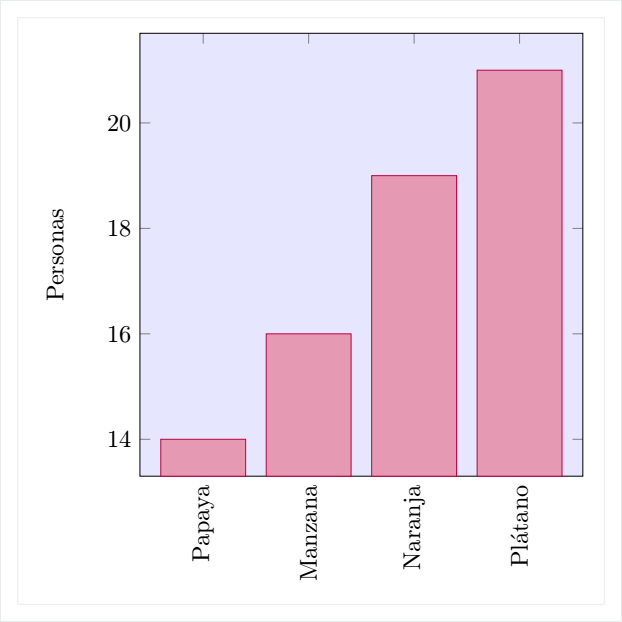
\includegraphics[width=\linewidth]{../images/imagen_barras_frutas02.png}
			\end{parts}
		\end{multicols}
	}

	%% \addcontentsline{toc}{subsubsection}{Gráficas circulares}
	%% \subsubsection*{Gráficas circulares}

	\questionboxed[2]{Los resultados de una encuesta se muestran en la siguiente gráfica de barras:

		\begin{multicols}{2}
			\begin{parts}\normalsize
				\part ¿Cuántas personas participaron en la encuesta? \fillin[140][1.5cm]
				\part  ¿Cuál es la fruta menos preferida por las personas? \fillin[uva][1.5cm]
				\part  ¿Cuál es la fruta preferida por las personas? \fillin[manzana][1.5cm]
				\part ¿Cuántas personas prefieren a las \textit{manzanas}.\fillin[40][1.5cm]
				\part ¿Cuántas personas prefieren a las \textit{uvas}.\fillin[28][1.5cm]
				\part ¿Cuántas personas prefieren a las \textit{naranjas}.\fillin[35][1.5cm]

				\columnbreak%

				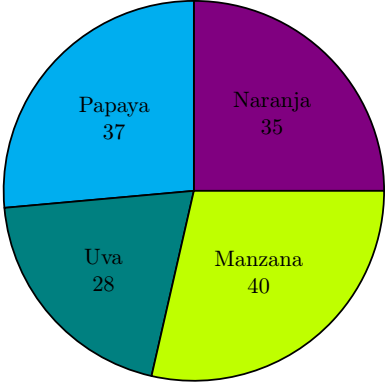
\includegraphics[width=0.8\linewidth]{../images/imagen_pie_frutas01.png}
			\end{parts}
		\end{multicols}

	}

	\addcontentsline{toc}{subsubsection}{Probabilidad}
	\subsubsection*{Probabilidad}
	\questionboxed[2]{Resuelve los siguientes problemas:

	\begin{multicols}{2}

		\begin{parts}
			% \part En una urna hay 10 pelotas azules, 5 verdes, 15 blancas y 20 negras. Calcula la probabilidad de sacar una pelota negra.

			% \begin{solutionbox}{1.5cm}
			% \end{solutionbox}

			\part Si se lanzan tres monedas al aire, calcula la probabilidad de que caiga puro sol.

			\begin{solutionbox}{2.5cm}
			\end{solutionbox}

			\part En una urna hay 8 pelotas moradas, 12 naranjas, 7 rojas, 11 azules y 7 blancas. Calcula la probabilidad de sacar una pelota negra.

			\begin{solutionbox}{1.5cm}
			\end{solutionbox}
		\end{parts}
	\end{multicols}
	}

	\addcontentsline{toc}{subsection}{Razones y proporciones}
	\subsection*{Razones y proporciones}
	%% \addcontentsline{toc}{subsubsection}{Razones 1}
	%% \subsubsection*{Razones 1}
	%% \addcontentsline{toc}{subsubsection}{Razones 2}
	%% \subsubsection*{Razones 2}

	\questionboxed[2]{Resuelve los siguientes problemas:

		\begin{multicols}{2}
			\begin{parts}
				% \part El perímetro de una cancha de fútbol mide 432 metros. Si la razón entre el ancho y el largo es de 5:7, ¿cuánto mide el largo de la cancha? \hfill\fillin[126][2cm]
				% \part En un salón, la razón entre la cantidad de mujeres y hombres es 7:8. Si hay un total de 45 alumnos entre hombres y mujeres, ¿cuántos son hombres? \hfill\fillin[21][2cm]
				% \part En un salón, la razón entre la cantidad de hombres y mujeres es 3:2. Si hay un total de 40 alumnos entre hombres y mujeres, ¿cuántos hombres hay? \hfill\fillin[24][2cm]
				\part Un fontanero y su ayudante reciben la cantidad de 2700 pesos por la instalación de equipo sanitario, si se reparten el dinero en razón de 7:2 respectivamente, ¿cuánto dinero recibirá el ayudante? \hfill\fillin[600][2cm]
				\part El perímetro de una cancha de fútbol mide 533 metros. Si la razón entre el ancho y el largo es de 6:7, ¿cuánto mide el ancho de la cancha? \hfill\fillin[123][2cm]
			\end{parts}
		\end{multicols}
	}


	%% \addcontentsline{toc}{subsubsection}{Encontrando el valor de x}
	%% \subsubsection*{Encontrando el valor de x}

	\questionboxed[2]{Calcula el valor de $x$ en las siguientes proporciones:

		\begin{multicols}{2}
			\begin{parts}
				% \part $ 2.6:7.8=3:x$ \fillin[$9$][1cm]
				\part $ x:4=15:6$ \fillin[$10$][1cm]
				\part $ 7.4:x=3.7:0.5$ \fillin[$1$][1cm]
				\part $ 49:56=x:8$ \fillin[$7$][1cm]
				\part $ 8:3.2=7.5:x$ \fillin[$3$][1cm]
			\end{parts}
		\end{multicols}
	}


	%% \addcontentsline{toc}{subsubsection}{Proporción directa}
	%% \subsubsection*{Proporción directa}
		%% \addcontentsline{toc}{subsubsection}{Proporción inversa}
	%% \subsubsection*{Proporción inversa}

	\questionboxed[2]{Resuelve los siguientes problemas:

		\begin{multicols}{2}
			\begin{parts}
				% \part Una máquina fabrica 400 tornillos en 5 horas, ¿cuánto tardará en fabricar 1,200 tornillos?
				% \fillin[$15$][1cm]

				\part Un grifo tiene un caudal de salida de 18 litros por minuto y tarda 14 horas en llenar un tanque. ¿Cuánto tardaría si el caudal fuera de 7 litros por minuto?
				\fillin[$36$][1cm]

				% \part Por 3 horas de trabajo Alberto ha cobrado 420 pesos. ¿Cuánto cobrará por 8 horas?
				% \fillin[$1120$][1cm]

				\part Un tinaco con 3 grifos tarda en llenarse 24 horas, ¿cuánto tardará en llenarse con 4 grifos?
				\fillin[$18$][1cm]

				% \part Un camión que viaja a 60 kilómetros por hora tarda 40 minutos en cubrir cierto recorrido, ¿cuánto tardará un coche que viaja a 150 kilómetros por hora?
				% \fillin[$16$][1cm]

				\part Si 12 vacas se comen un granero lleno de paja en 80 días, ¿cuánto tardarán en comerse la misma cantidad de paja 30 vacas?
				\fillin[$32$][1cm]

				% \part Una sandía cuesta 30 pesos, si Juan ha comprado 6 sandías, ¿cuánto ha pagado en total Juan?
				% \fillin[$180$][1cm]

				\part Diez pintores tardan 16 días en pintar una casa, ¿cuánto tiempo tardarán en hacerlo 8 pintores?
				\fillin[$20$][1cm]

				% \part Un corredor de maratón ha avanzado 2.4 kilómetros en 8 minutos. Si mantiene su velocidad constante, ¿cuánto tardará en completar los 42 kilómetros del maratón?
				% \fillin[$140$][1cm]
			\end{parts}
		\end{multicols}
	}


	\addcontentsline{toc}{subsection}{Círculo}
	\subsection*{Círculo}
	\addcontentsline{toc}{subsubsection}{Diámetro de un círculo}
	\subsubsection*{Diámetro de un círculo}
	\addcontentsline{toc}{subsubsection}{Radio de un círculo}
	\subsubsection*{Radio de un círculo}

	\questionboxed[2]{Contesta las siguientes preguntas:

		\begin{multicols}{2}
			\begin{parts}
				\part ¿Cuál es el diámetro de un círculo que tiene un radio de 21.98?

				\begin{solutionbox}{1cm}
					\fillin[43.96][0cm]
				\end{solutionbox}

				\part ¿Cuál es el diámetro de un círculo que tiene un radio de 39.21?

				\begin{solutionbox}{1cm}
					\fillin[78.42][0cm]
				\end{solutionbox}

				\part ¿Cuál es el diámetro de un círculo que tiene un radio de 6.7?

				\begin{solutionbox}{1cm}
					\fillin[13.4][0cm]
				\end{solutionbox}

				\part ¿Cuál es el radio de un círculo que tiene un diámetro de 88.28?

				\begin{solutionbox}{1cm}
					\fillin[44.19][0cm]
				\end{solutionbox}

			\end{parts}
		\end{multicols}
	}

	\addcontentsline{toc}{subsubsection}{Perímetro}
	\subsubsection*{Perímetro}
	\addcontentsline{toc}{subsubsection}{Área}
	\subsubsection*{Área}

	\questionboxed[2]{Calcula el perímetro y área de los siguientes círculos:

		\begin{multicols}{3}
			\begin{parts}

				\part 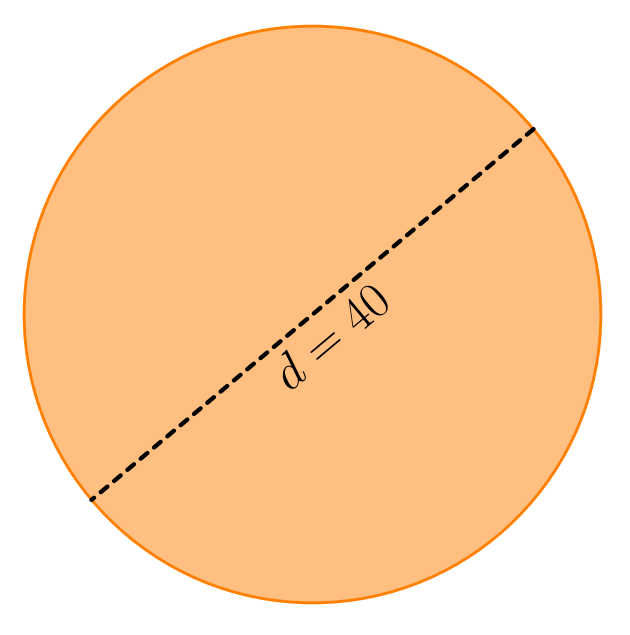
\includegraphics[width=0.7\linewidth]{../images/circulo01.png}\\
				\normalsize Perímetro: \fillin[62.8][0.3in]  Área: \fillin[1256][0.3in]

				\begin{solutionbox}{1.2cm}
					% $P=8\pi=8(3.14)=25.12$ \\
					% $A=\pi(4)^2=3.14(4)^2=50.24$
				\end{solutionbox}

				\part 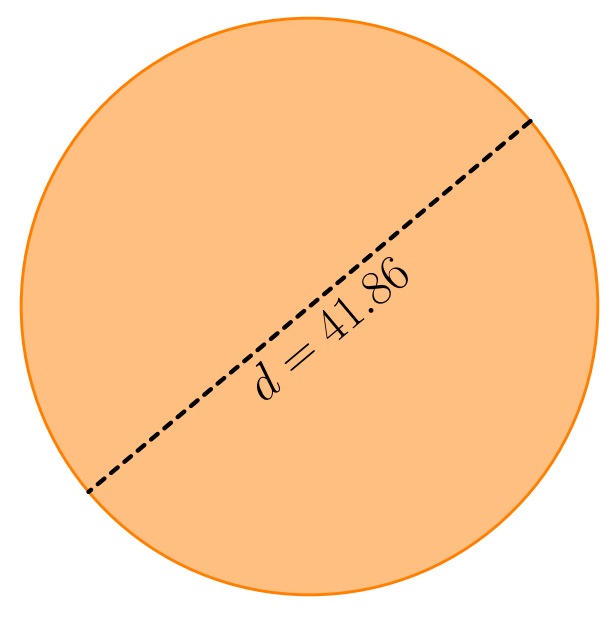
\includegraphics[width=0.7\linewidth]{../images/circulo02.png}\\
				\normalsize Perímetro: \fillin[131.51][0.3in]  Área: \fillin[1376.22][0.3in]

				\begin{solutionbox}{1.2cm}
					% $P=2\pi r=2(3.14)(9.3)=58.4$ \\
					% $A=\pi r^2=3.14(9.3)^2=271.57$
				\end{solutionbox}

				\part 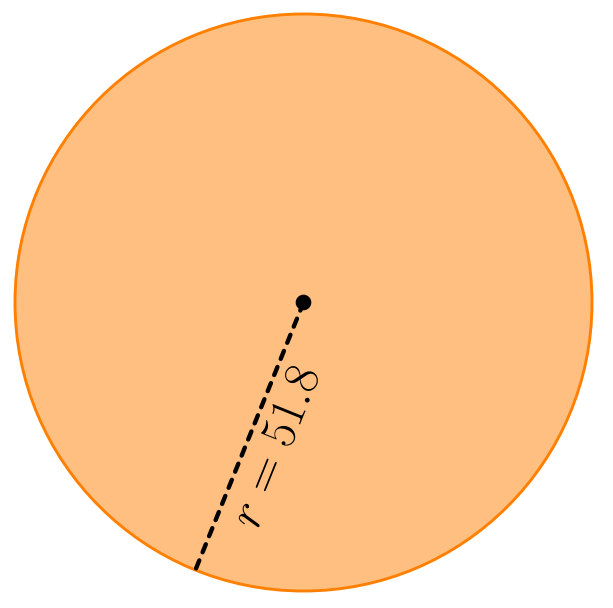
\includegraphics[width=0.7\linewidth]{../images/circulo03.png}\\
				\normalsize Perímetro: \fillin[325.47][0.3in]  Área: \fillin[8429.65][0.3in]

				\begin{solutionbox}{1.2cm}
					% $P=2\pi r=2(3.14)(12)=75.36$ \\
					% $A=\pi r^2=3.14(12)^2=452.16$
				\end{solutionbox}

				\part 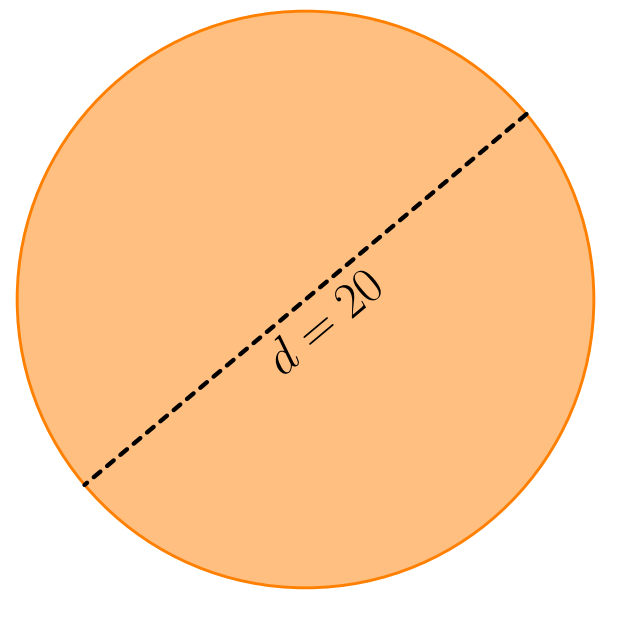
\includegraphics[width=0.7\linewidth]{../images/circulo04.png}\\
				\normalsize Perímetro: \fillin[62.8][0.3in]  Área: \fillin[314][0.3in]

				\begin{solutionbox}{1.2cm}
					% $P=8\pi=8(3.14)=25.12$ \\
					% $A=\pi(4)^2=3.14(4)^2=50.24$
				\end{solutionbox}

				\part 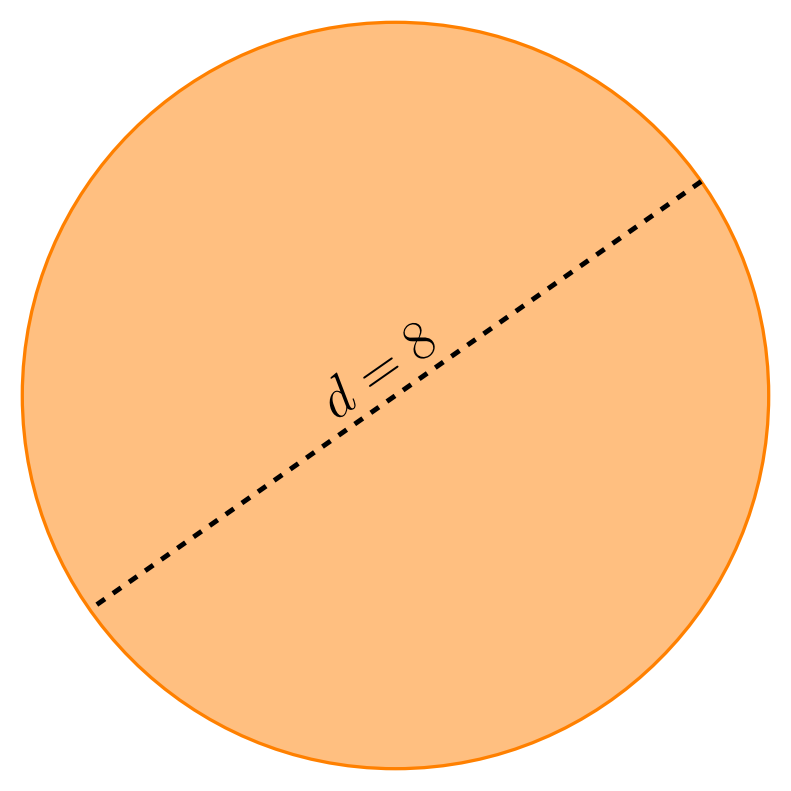
\includegraphics[width=0.7\linewidth]{../images/circulo05.png}\\
				\normalsize Perímetro: \fillin[25.12][0.3in]  Área: \fillin[50.24][0.3in]

				\begin{solutionbox}{1.2cm}
					% $P=2\pi r=2(3.14)(9.3)=58.4$ \\
					% $A=\pi r^2=3.14(9.3)^2=271.57$
				\end{solutionbox}

				\part 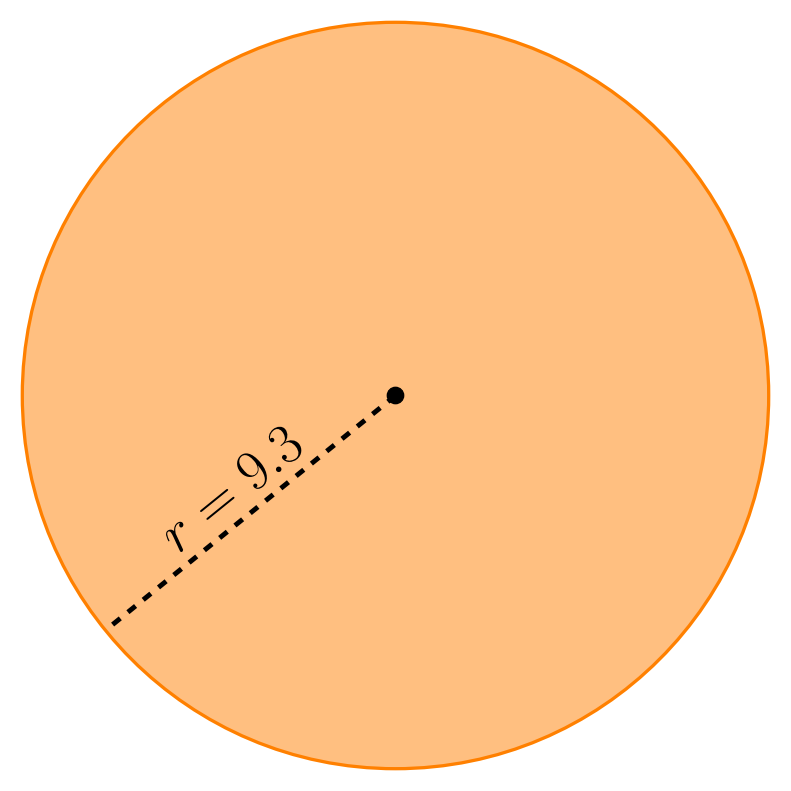
\includegraphics[width=0.7\linewidth]{../images/circulo06.png}\\
				\normalsize Perímetro: \fillin[58.404][0.3in] Área: \fillin[271.57][0.3in]

				\begin{solutionbox}{1.2cm}
					% $P=2\pi r=2(3.14)(12)=75.36$ \\
					% $A=\pi r^2=3.14(12)^2=452.16$
				\end{solutionbox}
			\end{parts}
		\end{multicols}
	}

	\addcontentsline{toc}{subsubsection}{Resolución de problemas}
	\subsubsection*{Resolución de problemas}

	\addcontentsline{toc}{subsection}{Figuras geométricas}
	\subsection*{Figuras geométricas}
	\addcontentsline{toc}{subsubsection}{Nombre de figuras}
	\subsubsection*{Nombre de figuras}

	\questionboxed[2]{Escribe sobre la línea el nombre que recibe cada figura geométrica de acuerdo con su número de lados:

		\begin{multicols}{3}
			\begin{parts}
				\part 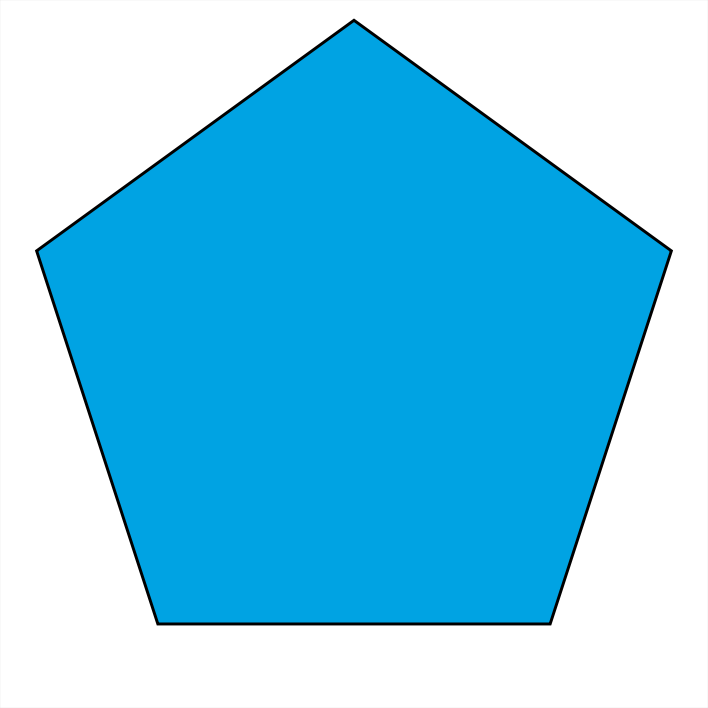
\includegraphics[width=75px]{../images/pentagono_azul.png}  \fillin[pentágono][0.75in]
				\part 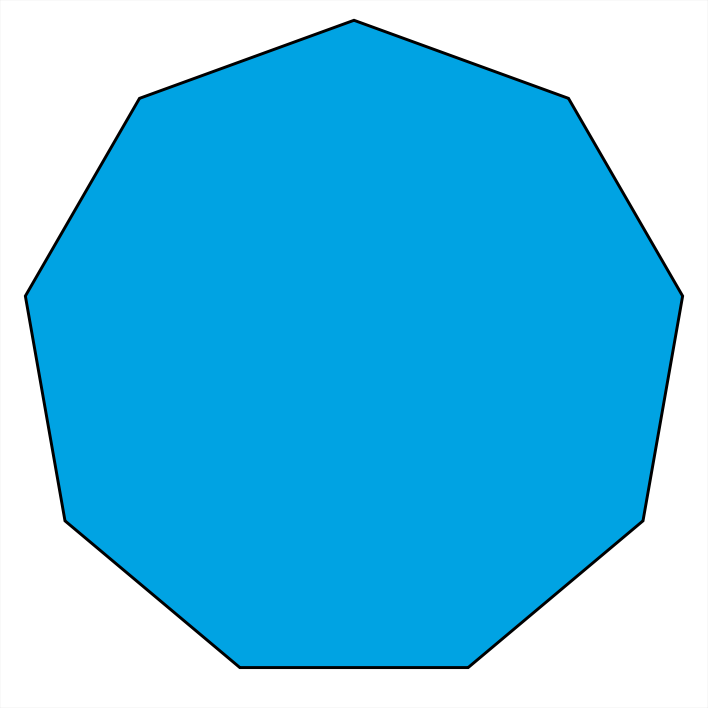
\includegraphics[width=75px]{../images/nonagono_azul.png}   \fillin[nonágono][0.75in]
				\part 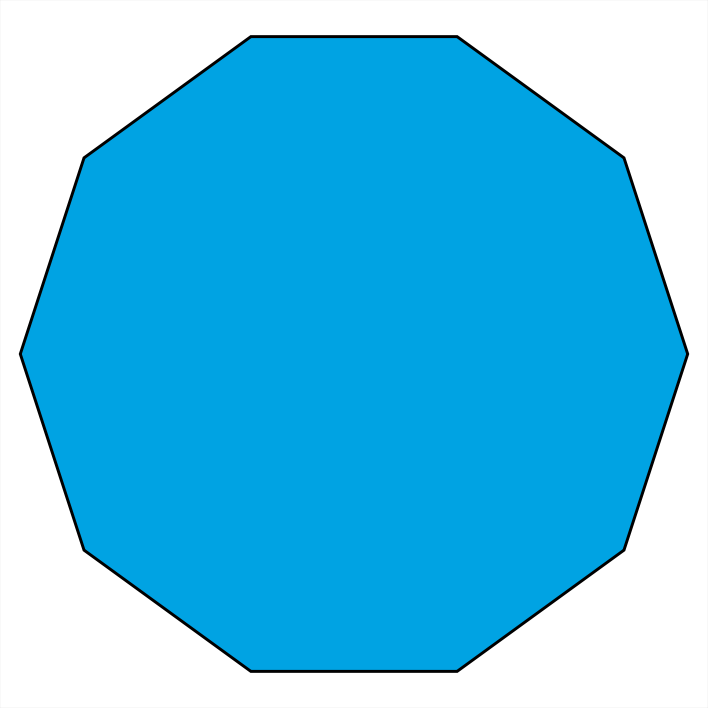
\includegraphics[width=75px]{../images/decagono_azul.png}   \fillin[decágono][0.75in]
				\part 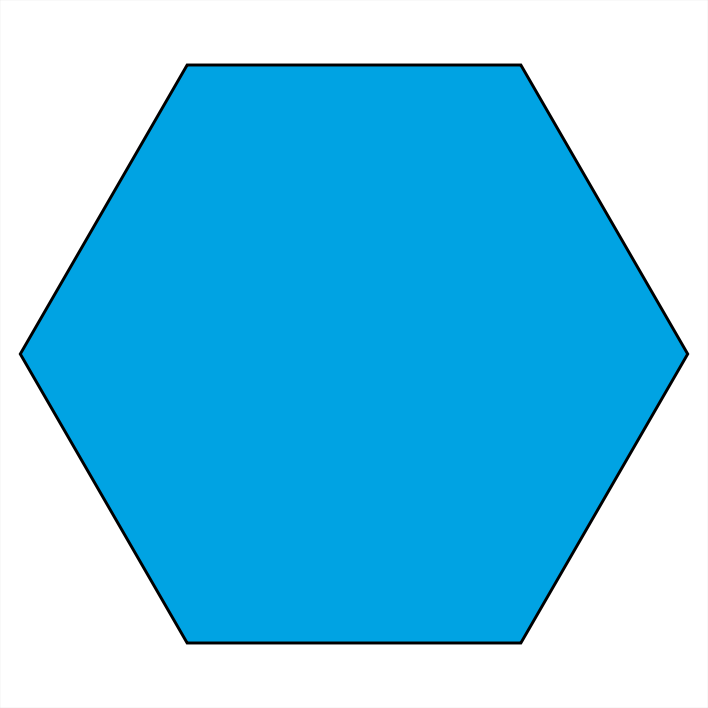
\includegraphics[width=75px]{../images/hexagono_azul.png}   \fillin[hexágono][0.75in]
				\part 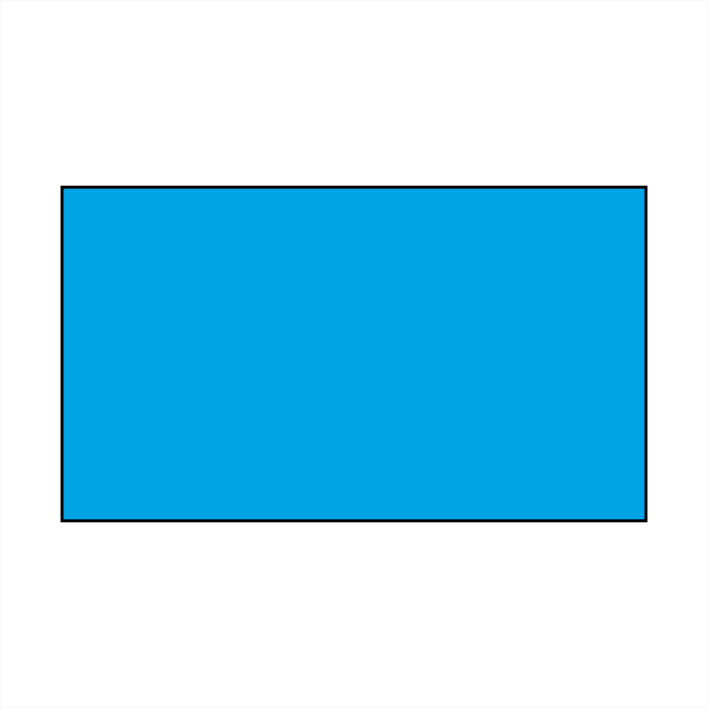
\includegraphics[width=75px]{../images/rectangulo_azul.png} \fillin[rectángulo][0.75in]
				\part 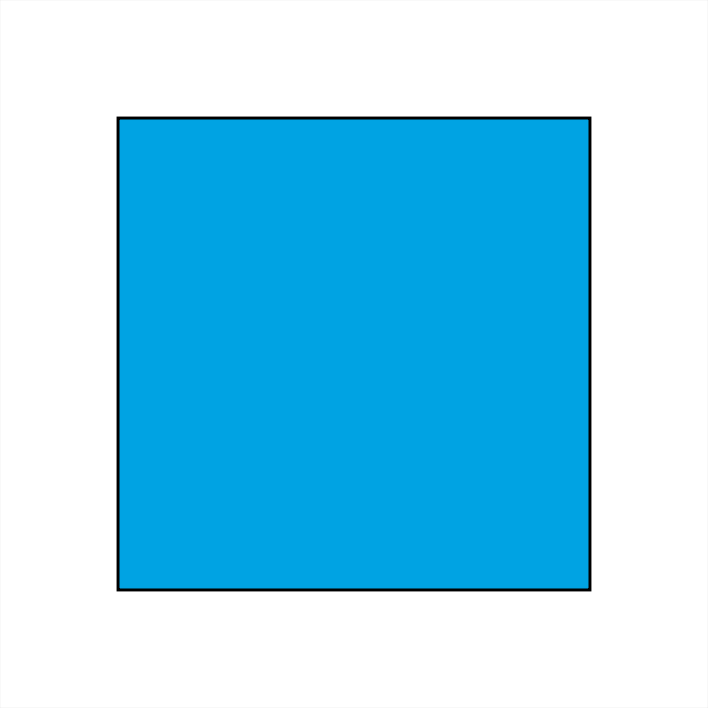
\includegraphics[width=75px]{../images/cuadrado_azul.png}   \fillin[cuadrado][0.75in]
			\end{parts}
		\end{multicols}
	}

	%% \addcontentsline{toc}{subsubsection}{Elementos de figuras}
	%% \subsubsection*{Elementos de figuras}


	\addcontentsline{toc}{subsubsection}{Perímetro}
	\subsubsection*{Perímetro}

	\questionboxed[2]{Contesta las preguntas sobre perímetros de figuras geométricas

		\begin{multicols}{2}
			\begin{parts}
				\part ¿Cuál es el perímetro de un rectángulo cuya base mide 38 y su altura mide 19?

				\begin{solutionbox}{1cm}
					\[P=38+19+38+19=\color{red}114\]
				\end{solutionbox}

				\part ¿Cuál es el perímetro de un cuadrado que sus lados miden 5?

				\begin{solutionbox}{1cm}
					\[P=5+5+5+5=\color{red}20\]
				\end{solutionbox}

				\part ¿Cuál es el perímetro de un pentágono que sus lados miden 18?

				\begin{solutionbox}{1cm}
					\[P=18 \times 5=\color{red}90\]
				\end{solutionbox}

				% \part ¿Cuál es el perímetro de un octágono que sus lados miden 15?

				% \begin{solutionbox}{1cm}
				% 	\[P=15 \times 8=\color{red}120\]
				% \end{solutionbox}

				\part ¿Cuál es el perímetro de un rombo que sus lados miden 16?

				\begin{solutionbox}{1cm}
					\[P=16 \times 4=\color{red}64\]
				\end{solutionbox}

			\end{parts}
		\end{multicols}
	}

	\addcontentsline{toc}{subsubsection}{Área}
	\subsubsection*{Área}

	\questionboxed[2]{Contesta las preguntas sobre áreas de figuras geométricas

		\begin{multicols}{2}
			\begin{parts}
				\part ¿Cuál es el área de un triángulo cuya base mide 18 y su altura mide 11?

				\begin{solutionbox}{1.5cm}
					\[A=\dfrac{18 \times 11}{2}=\color{red}99\]
				\end{solutionbox}


				\part ¿Cuál es el área de un cuadrado que sus lados miden 29?

				\begin{solutionbox}{1.5cm}
					\[A=29 \times 29=\color{red}841\]
				\end{solutionbox}

			\end{parts}
		\end{multicols}
	}

	\addcontentsline{toc}{subsubsection}{Resolución de problemas}
	\subsubsection*{Resolución de problemas}

	\questionboxed[2]{Resuelve los siguientes problemas:

		\begin{multicols}{2}
			\begin{parts}
				% \part Alejandro quiere poner una barda alrededor de un terreno cuadrangular que mide 22 metros por lado. ¿Cuánta barda necesitará Alejandro para poner barda en todo el terreno?

				% \begin{solutionbox}{1cm}
				% 	\fillin[88][0in]
				% \end{solutionbox}

				\part Para darle mantenimiento a una alberca olímpica se pone cinta alrededor de esta. Si la alberca tiene 50 metros de largo y 25 metros de ancho, ¿cuánta cinta se necesita para darle la vuelta a la alberca?

				\begin{solutionbox}{1cm}
					\fillin[150][0in]
				\end{solutionbox}


				% \part Bruno corre todos los días en un parque de forma rectangular el cual mide 75 metros de largo y 40 metros de ancho. ¿Cuántos metros corre Bruno por una vuelta?

				% \begin{solutionbox}{1cm}
				% 	\fillin[230][0in]
				% \end{solutionbox}

				\part Bruno corre todos los días en un parque de forma rectangular el cual mide 50 metros de largo y 28 metros de ancho. Si al día le da 4 vueltas al parque, ¿cuántos metros habrá corrido en total Bruno?

				\begin{solutionbox}{1cm}
					\fillin[624][0in]
				\end{solutionbox}
			\end{parts}
		\end{multicols}
	}

	\addcontentsline{toc}{subsection}{Cuerpos geométricos}
	\subsection*{Cuerpos geométricos}
	%% \addcontentsline{toc}{subsubsection}{Nombre de cuerpos geométricos}
	%% \subsubsection*{Nombre de cuerpos geométricos}
	%% \addcontentsline{toc}{subsubsection}{Elementos de cuerpos geométricos}
	%% \subsubsection*{Elementos de cuerpos geométricos}
	%% \addcontentsline{toc}{subsubsection}{Área lateral}
	%% \subsubsection*{Área lateral}
	%% \addcontentsline{toc}{subsubsection}{Área total}
	%% \subsubsection*{Área total}
	%% \addcontentsline{toc}{subsubsection}{Volumen}
	%% \subsubsection*{Volumen}

	\questionboxed[4]{Calcula el volumen, el área lateral y el área total de las siguientes figuras:
    
	\begin{multicols}{2}
            \begin{parts}
                % \part 
				% 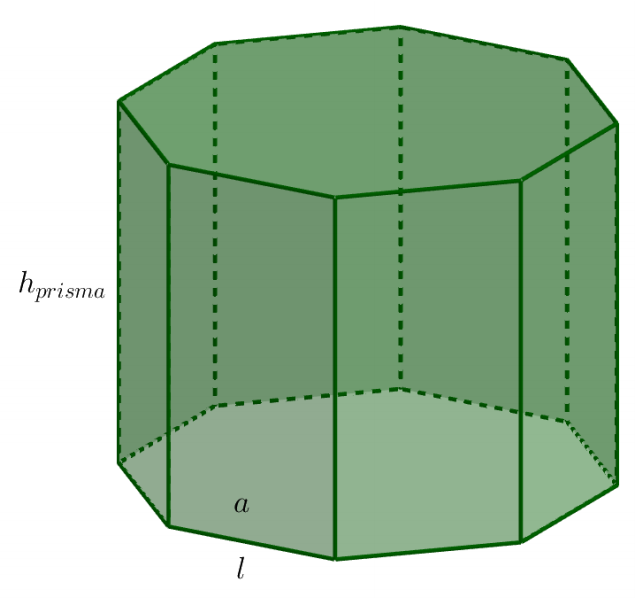
\includegraphics[width=0.6\linewidth]{mex_0025.png}\\
                % Prisma cuyos lados "l" de la base miden 8 cm y la altura "h" mide 21 cm.\\
                % Volumen: \fillin[u$^3$][0.4in] \\A. Lateral: \fillin[][0.4in] \\ A. Total: \fillin[u$^2$][0.4in]

                % \part 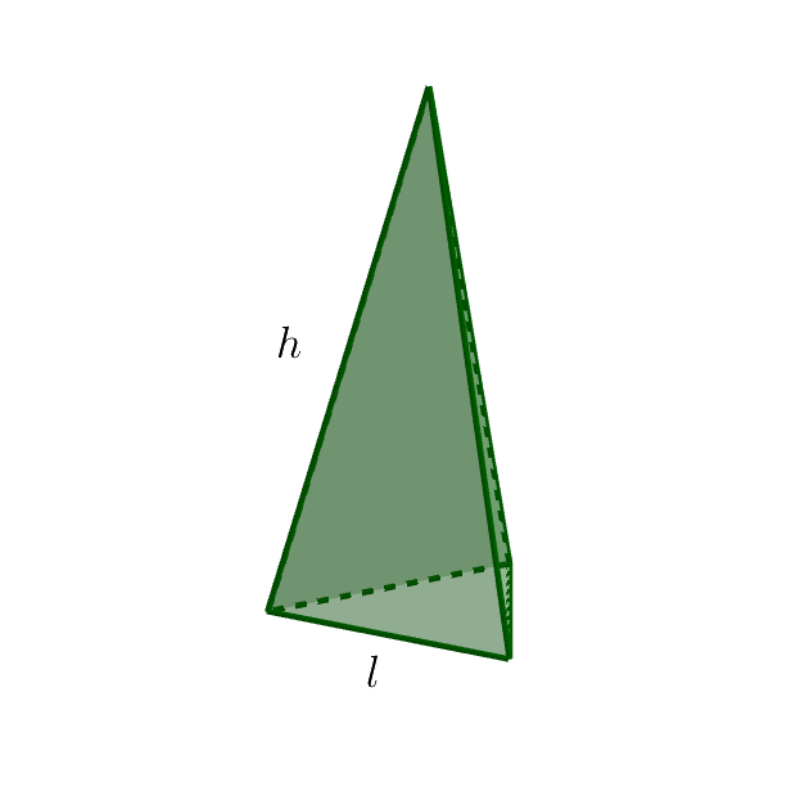
\includegraphics[width=\linewidth]{mex_0023.png}
                % Pirámide cuyos lados "l" de la base miden 13 cm y la altura "h" mide 42 cm.\\
                % Volumen: \fillin[$$ u$^3$][0.4in] \\A. Lateral: \fillin[$$ u][0.4in] \\ A. Total: \fillin[$$ u$^2$][0.4in]

                \part 
				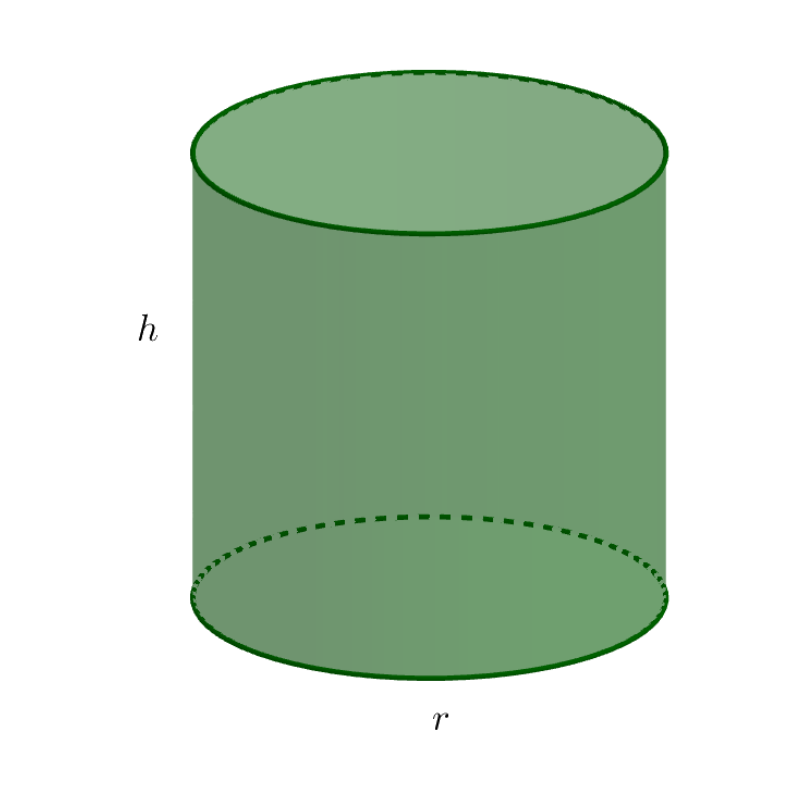
\includegraphics[width=0.6\linewidth]{mex_0024.png}\\
                Cilindro con altura $h=17$ cm y un radio $r=4$ cm.\\
              \small  Volumen: \fillin[u$^3$][0.4in] \\A. Lateral: \fillin[][0.4in] \\ A. Total: \fillin[u$^2$][0.4in]

                % \part 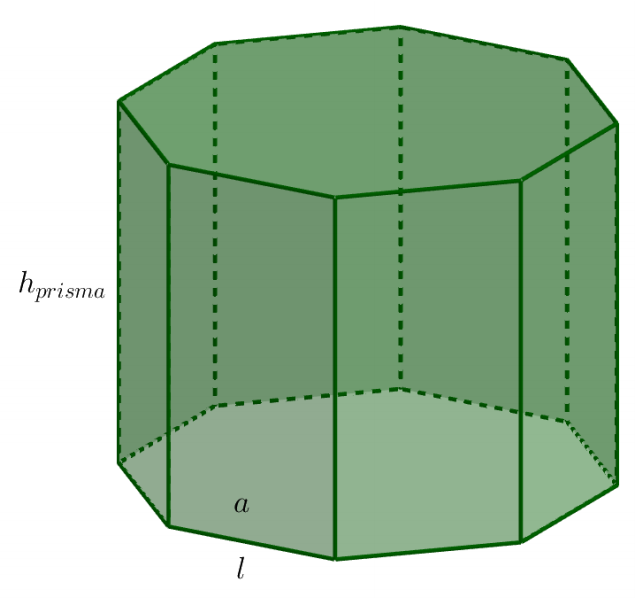
\includegraphics[width=\linewidth]{mex_0025.png}
                % Volumen: \fillin[$$ u$^3$][0.4in] \\A. Lateral: \fillin[$$ u][0.4in] \\ A. Total: \fillin[$$ u$^2$][0.4in]

                \part 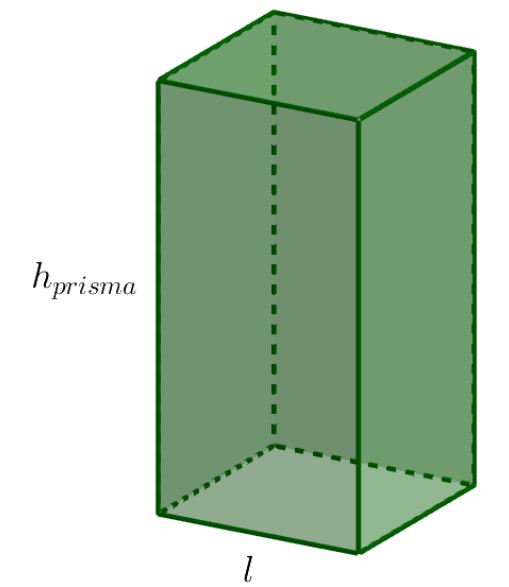
\includegraphics[width=0.6\linewidth]{mex_0026.png}\\
                Prisma cuyos lados "l" de la base miden 15 cm y la altura "h" mide 24 cm.\\
               \small Volumen: \fillin[u$^3$][0.4in] \\A. Lateral: \fillin[][0.4in] \\ A. Total: \fillin[u$^2$][0.4in]

                \part 
				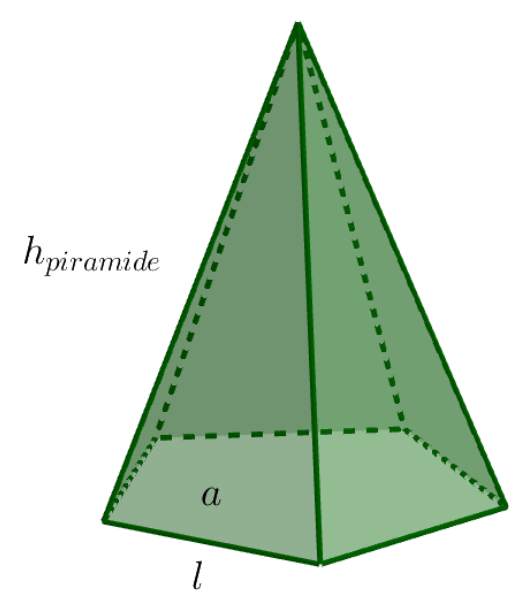
\includegraphics[width=0.6\linewidth]{mex_0027.png}\\
                Pirámide de 19 cm de altura cuya base es un pentágono cuyos lados "l" miden 8 cm y su apotema "a" mide 5 cm.\\
              \small  Volumen: \fillin[u$^3$][0.4in] \\A. Lateral: \fillin[][0.4in] \\ A. Total: \fillin[u$^2$][0.4in]

                % \part 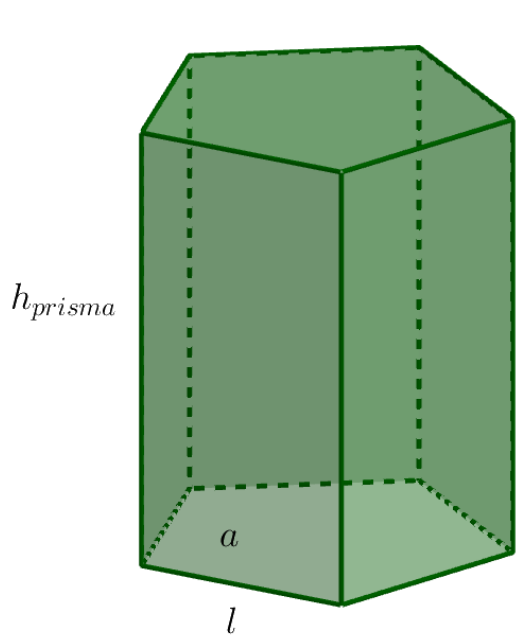
\includegraphics[width=\linewidth]{mex_0028.png}
                % Volumen: \fillin[$$ u$^3$][0.4in] \\A. Lateral: \fillin[$$ u][0.4in] \\ A. Total: \fillin[$$ u$^2$][0.4in]

                \part 
				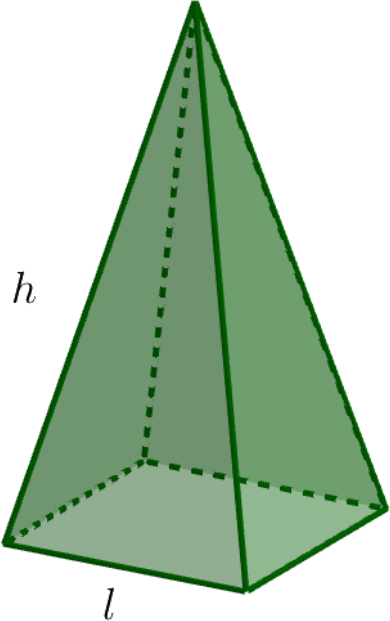
\includegraphics[width=0.6\linewidth]{mex_0029.png}\\
                Pirámide cuyos lados "l" de la base miden 16 cm y la altura "h" mide 27 cm.\\
               \small Volumen: \fillin[u$^3$][0.4in] \\A. Lateral: \fillin[][0.4in] \\ A. Total: \fillin[u$^2$][0.4in]

                % \part 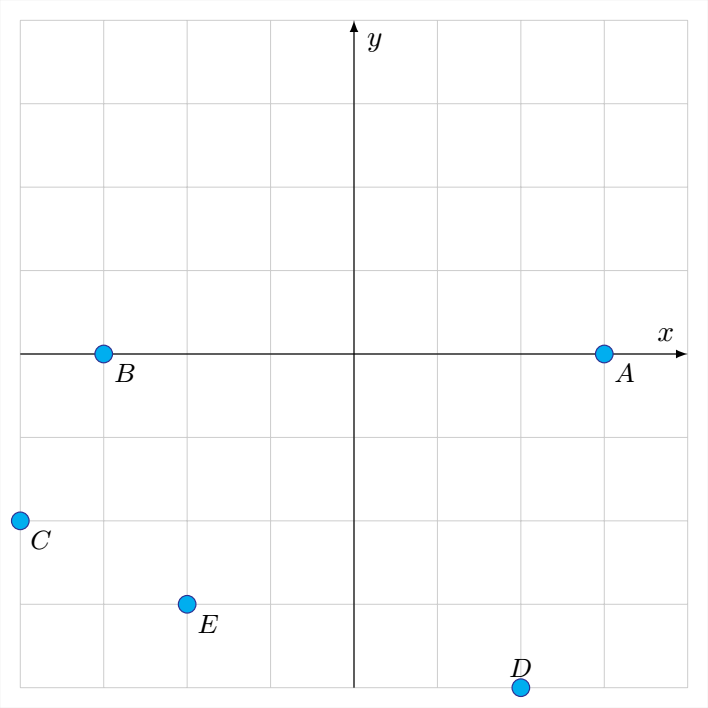
\includegraphics[width=\linewidth]{mex_0030.png}
                % Volumen: \fillin[$$ u$^3$][0.4in] \\A. Lateral: \fillin[$$ u][0.4in] \\ A. Total: \fillin[$$ u$^2$][0.4in]
            \end{parts}
        \end{multicols}
    }


	\addcontentsline{toc}{subsection}{Sistema de unidades}
	\subsection*{Sistema de unidades}
	\addcontentsline{toc}{subsubsection}{Operaciones con múltiplos de 10}
	\subsubsection*{Operaciones con múltiplos de 10}

	\questionboxed[2]{Realiza las siguientes operaciones:

		\begin{multicols}{2}
			\begin{parts}
				% \part $ 93.2 \times 1000=$   \fillin[93200][0.5in]
				\part $ 84.2 \times 100=$   \fillin[8420][0.5in]
				\part $ 66.472 \times 10000=$   \fillin[664720][0.5in]
				\part $ 192.3 \times 10=$   \fillin[1923][0.5in]
				\part $ 26.9 \times 1000=$   \fillin[26900][0.5in]
				\part $ 81.674 \times 100000=$   \fillin[8167400][0.5in]
				\part $ 1.2 \times 1000=$   \fillin[1200][0.5in]
				\part $ 7.8 \times 10=$   \fillin[78][0.5in]
				\part $ 38093 \divisionsymbol 10=$   \fillin[3809.3][0.5in]
				\part $ 28 \divisionsymbol 1000=$   \fillin[0.028][0.5in]
				\part $ 44567 \divisionsymbol 100=$   \fillin[445.67][0.5in]
				\part $ 678 \divisionsymbol 1000=$   \fillin[0.678][0.5in]
				\part $ 7.1 \divisionsymbol 10=$   \fillin[0.71][0.5in]
				\part $ 51 \divisionsymbol 100=$   \fillin[0.51][0.5in]
				\part $ 3.9 \divisionsymbol 100=$   \fillin[0.039][0.5in]
				% \part $ 2.4 \divisionsymbol 100=$   \fillin[0.024][0.5in]
				% \part $ 34 \divisionsymbol 10=$   \fillin[3.4][0.5in]
				% \part $ 6.3 \divisionsymbol 10000=$   \fillin[0.00063][0.5in]
			\end{parts}
		\end{multicols}
	}

	\addcontentsline{toc}{subsubsection}{Unidades de longitud}
	\subsubsection*{Unidades de longitud}
	\addcontentsline{toc}{subsubsection}{Unidades de masa}
	\subsubsection*{Unidades de masa}
	\addcontentsline{toc}{subsubsection}{Unidades de capacidad}
	\subsubsection*{Unidades de capacidad}
	\questionboxed[2]{Realiza las siguientes conversiones de unidades de longitud y masa:

		\begin{multicols}{2}
			\begin{parts}\normalsize
				\part De 157 kilómetros a hectómetros. \hfill \fillin[1570][0.6in] hm
				\part De 25 centímetros a milímetros.  \hfill \fillin[250][0.6in] mm
				% \part De 27 kilómetros a decámetros.   \hfill \fillin[2700][0.6in] Dm
				% \part De 27 hectolitros a decilitros. \hfill \fillin[27000][0.6in] dL
				% \part De 17 kilómetros a hectómetros.  \hfill \fillin[170][0.6in] hm
				% \part De 69 kilómetros a centímetros.  \hfill \fillin[6900000][0.6in] cm
				% \part De 59 decímetros a centímetros.  \hfill \fillin[590][0.6in] cm
				% \part De 26 metros a decímetros.       \hfill \fillin[260][0.6in] dm
				% \part De 8 mililitros a centilitros. \hfill \fillin[0.8][0.6in] cL
				% \part De 4 kilómetros a milímetros.    \hfill \fillin[4000000][0.6in] mm
				% \part De 135 kilómetros a decámetros.  \hfill \fillin[13500][0.6in] Dm
				% \part De 112 kilómetros a hectómetros. \hfill \fillin[1120][0.6in] hm
				\part De 205 gramos a decigramos    \hfill \fillin[2050][0.5in] dg
				\part De 25 kilogramos a gramos     \hfill \fillin[25000][0.5in] g
				\part De 1094 mililitros a decilitros. \hfill \fillin[10.94][0.6in] dL
				\part De 58 kilogramos a gramos     \hfill \fillin[58000][0.5in] g
				\part De 45 decagramos a gramos     \hfill \fillin[450][0.5in] g
				\part De 134 gramos a decigramos    \hfill \fillin[1340][0.5in] dg
				\part De 702 mililitros a decilitros. \hfill \fillin[7.02][0.6in] dL
				\part De 282 gramos a miligramos    \hfill \fillin[282000][0.5in] mg
				\part De 117 decagramos a gramos    \hfill \fillin[1170][0.5in] g
				\part De 17 decigramos a miligramos \hfill \fillin[1700][0.5in] mg
				\part De 115 gramos a centigramos   \hfill \fillin[11500][0.5in] cg
				\part De 62 gramos a miligramos     \hfill \fillin[62000][0.5in] mg
			\end{parts}
		\end{multicols}
	}

	\addcontentsline{toc}{subsubsection}{Unidades de área y volumen}
	\subsubsection*{Unidades de área y volumen}
	\questionboxed[2]{Convierte las siguientes unidades de área y volumen como se te pide:

		\begin{multicols}{2}
			\begin{parts}
				\part Convierte 8.03 metros cúbicos a milímetros cúbicos
				\part Convierte 8 kilómetros cuadrados a metros cuadrados
				\part Convierte 88 metros cuadrados a kilómetros cuadrados
				% \part Convierte 18 decámetros cúbicos a milímetros cúbicos
				\part Convierte 801 milímetros cuadrados a decámetros cuadrados
			\end{parts}
		\end{multicols}
	}


\end{questions}
\end{document}